\RequirePackage{fix-cm}
\documentclass[twocolumn]{svjour3}
\smartqed

\usepackage[T1]{fontenc}
\usepackage[utf8]{inputenc}
\usepackage{microtype}
\usepackage{amsmath,amssymb,booktabs,longtable,array,graphicx,xcolor}
\usepackage[hyphens]{url}
\usepackage[hidelinks]{hyperref}
\Urlmuskip=0mu plus 2mu\relax
\tolerance=2000
\hbadness=10000
\emergencystretch=3em
\raggedbottom

\journalname{Eur. Phys. J. C}

\newcommand{\pin}{p_{\mathrm{in}}}
\newcommand{\pout}{p_{\mathrm{out}}}
\newcommand{\deltap}{\Delta p}
\newcommand{\phys}{\mathrm{BB}}
\newcommand{\raw}{\mathrm{Raw}}
\newcommand{\learned}{\mathrm{PR}}
\newcommand{\simple}{\mathrm{Lin}}

\begin{document}

\title{Non-monotonic benefits of physical target centering in conditional models of pion momentum loss}
\titlerunning{Non-monotonic benefits of physical target centering in pion momentum loss}

\author{Xuansong Chang \and
        Yiran Xiao \and
        Chengtao Song}
\authorrunning{X. Chang et al.}

\institute{X. Chang \and Y. Xiao \and C. Song \at
              [Affiliation to be supplied by authors prior to portal upload] \\
              \email{[corresponding.author@institution.edu]}}

\date{Received: date / Accepted: date}

\maketitle

\begin{abstract}
A prescribed target representation can change the approximation problem faced
by a finite conditional density estimator even when the transformation is
invertible. We examine how physical target centering interacts with the
information directly available to a neural conditioner, using pion momentum
loss in silicon. Matched spline flows compare raw and Bethe--Bloch-centered
targets under no direct, two-bin, eight-bin and exact momentum inputs.
Exact momentum remains available to the physical center and support
calculation. Eighty training runs cover two training fractions and five paired
optimizer seeds. Models and prespecified analyses are frozen before generating two
500,000-event Geant4 catalogs. Mean centering gains peak at two-bin information
($0.0104$--$0.0112$ nat/event), while exact conditioning gives the best absolute
mean negative log-likelihood. The rise and fall around this peak occur for all
five seeds; the smaller final decline has one seed exception at 10\% training.
Positive overall gains coexist with regional likelihood losses and calibration
trade-offs. The stable intermediate peak shows a non-monotonic representation--information
interaction in the tested density-model design. The comparisons distinguish
relative centering benefit, absolute prediction quality and the distribution
of gains across physical conditions.
\keywords{conditional density estimation \and target representation \and normalizing flow \and conditioner information \and pion momentum loss}
\end{abstract}

\section{Introduction}
\label{sec:intro}

An invertible target transformation preserves the ideal conditional density
problem, but can change what a finite estimator must learn. A prescribed
center $c(V,W)$ replaces a response $Y$ with the residual $Y-c(V,W)$.
When the density network has complete conditions $(V,W)$, this is a change of
coordinates. When its inputs are restricted, the center also supplies a fixed
dependence on information that the residual network cannot freely adjust.
The scientific question is: \emph{When does prescribed physical target centering
help conditional density estimation, and how does its benefit depend on the
information available to the neural conditioner?}

Exact physical inputs can enter a surrogate through a prescribed baseline,
the neural conditioner, or both. We use controlled coarsening of the neural
inputs to examine how these two information paths interact in a finite
conditional density model. The experiment retains exact incident momentum in
the center and support calculation, while providing the network with no direct,
two-bin, eight-bin or exact momentum information. This design examines how
prescribed and learned information paths interact under a matched nominal
architecture and training budget.

The application is simulated pion momentum loss in silicon. Thin absorbers
motivate a distributional description beyond mean stopping
power~\cite{Bichsel1988,PDG2025}; Geant4 supplies the transport
reference~\cite{Agostinelli2003,Allison2006,Allison2016}. A nominal Bethe--Bloch prediction defines
the target center, and conditional spline flows provide the matched
comparison tool. Both the physical center and the raw-target baseline use
the same nominal network architecture and optimization budget.

We separate three evaluation questions: how much centering improves its raw
baseline, which complete predictor has the best absolute likelihood, and
whether improvement is shared across physical regions. The relative gain
peaks at intermediate momentum information, exact conditioning yields the
lowest mean NLL, and aggregate gains coexist with local losses.
Two fresh simulation catalogs assess event variability after model selection
has ended, while paired optimizer seeds expose training variability. Together
these comparisons make information access an experimental axis for studying
the value of a prescribed representation. Complete numerical tables,
seed-sensitivity checks and implementation diagnostics are provided in the
Electronic Supplementary Material (Supplementary Sections S1--S5).

\section{Related work}
\label{sec:related_target_centering}

Physical knowledge enters learned models through several interfaces. Hybrid
process models combine mechanistic structure with learned quantities~\cite{PsichogiosUngar1992};
physics-informed neural networks use differential-equation residuals in the
objective~\cite{RaissiPerdikarisKarniadakis2019}; APHYNITY learns a constrained
correction to incomplete dynamics~\cite{YinEtAl2021}. These approaches motivate
studying which part of a prediction problem is assigned to the physical
description and which part remains statistical. Here the physical prescription
defines the response coordinate, and the flow learns its conditional density.

Residual targets have a direct precedent in $\Delta$-machine learning, where
a learned correction augments an inexpensive quantum-chemical baseline~\cite{RamakrishnanEtAl2015}.
Conditional transformation models extend response transformation to
distributional regression by estimating transformations that depend on
explanatory variables~\cite{HothornKneibBuhlmann2014}. These lines connect
baseline correction with conditional distribution modeling. Our center is
prescribed before flow fitting, so the experimental variable is the residual
task presented to a matched density estimator.

Response parameterization can affect both model adequacy and optimization.
Box and Cox studied transformations that make a simple regression and error
model appropriate, comparing likelihoods on the original response scale with
the Jacobian included~\cite{BoxCox1964}. PopArt changes target normalization
while compensating the output layer to preserve the unnormalized predictor,
relating normalization to modified squared-loss SGD updates~\cite{VanHasseltEtAl2016}.
For squared-loss kernel regression, target power across kernel eigenfunctions
links target--model alignment to generalization~\cite{CanatarBordelonPehlevan2021}.
Together these results show why an information-preserving coordinate choice
can still matter to a restricted learner. Our arms share a global target scale
and fit a residual offset, focusing the comparison on input-dependent centering.

Normalizing flows permit tractable density evaluation through change of
variables. Conditional masked autoregressive flows incorporate explanatory
inputs into their transformations~\cite{PapamakariosPavlakouMurray2017},
and neural spline flows provide monotone rational-quadratic maps with analytic
inverses~\cite{DurkanEtAl2019}. Tail fidelity and expressiveness also depend on
base-distribution structure, Lipschitz behavior, depth and numerical
conditioning~\cite{JainiKobyzevYuBrubaker2020,KoehlerMehtaRisteski2021}.
Numerical conditioning concerns the invertible map and its Jacobian, distinct
from the physical information supplied to the neural conditioner.

In high-energy physics, deep generative surrogates increasingly complement
detailed Monte Carlo detector transport~\cite{HashemiKrause2024}, with
conditional normalizing flows achieving high-fidelity shower and material-parameterized
response modeling~\cite{KrauseShih2023,ErdmannEtAl2025}. Conversely, in inverse
detector reconstruction, physics-constrained generative models have recently
recovered sub-crystal electromagnetic shower structure from coarse segmented
calorimeter readouts by enforcing low-order spatial-moment
constraints~\cite{LiuTung2026}. Charged-particle tracking frameworks likewise
combine fast analytic material-interaction formulas with stochastic straggling
descriptions~\cite{AiEtAl2022}. In such forward hybrid settings, an analytic
stopping-power reference can evaluate exact step kinematics directly, whereas a
learned residual model may operate on coarsened, tabulated or reduced
conditioning inputs.

These studies establish residual modeling, coordinate choice and flow-based
transport surrogates as relevant tools; they do not determine the ordering of
finite spline-flow NLLs under restricted neural inputs. Our contribution is
the controlled information-axis comparison for a prescribed physical target
center. Matched raw-target baselines separate centering benefit from the
absolute benefit of additional neural information, and regional evaluations
test how aggregate changes are distributed across the physical domain.


\section{Information paths and conditional density model}
\label{sec:model}

\subsection{Physical target and prescribed center}

The response is $Y=\Delta p=\pin-\pout$ in GeV/$c$ for the original
primary pion's first contiguous visit to a silicon slab, conditional on a
forward exit ($S=1$). Here $\pin$ is the generated incident momentum and
$\pout$ is the momentum magnitude at that visit's recorded exit. Eligibility
requires a recorded entry and downstream-face exit, $\pout>0$, and no
technical abort; later visits and secondary particles do not define this
target. Incident momenta span $0.3$--$1.0$ GeV/$c$, slab thicknesses $t$ are
$0.1$, $0.3$ and $1.0$ mm, and pion charge $q$ is $-1$ or $+1$.
Outcomes without a valid continuous target remain in the event ledger;
the density estimand conditions on $S=1$. The raw representation uses $c=0$.

For the physical reference, put $P=1000\pin$ in MeV/$c$,
$M_\pi=139.57039$ MeV/$c^2$, $M_e=0.51099895$ MeV/$c^2$,
$E=\sqrt{P^2+M_\pi^2}$, $\beta=P/E$, and $\gamma=E/M_\pi$. Then
\begin{align}
 T_{\max} &= \frac{2M_e\beta^2\gamma^2}
 {1+2\gamma M_e/M_\pi+(M_e/M_\pi)^2},\\
 S_{\mathrm{BB}} &= K\frac{Z}{A}\frac{q^2}{\beta^2}
 \left[\frac12\log\!\left(\frac{2M_e\beta^2\gamma^2T_{\max}}{I^2}\right)-\beta^2\right],
\end{align}
with $K=0.307075$ MeV cm$^2$/mol and $Z/A=14/(28.0855\,\mathrm{g/mol})$,
$\rho=2.329$ g/cm$^3$, and $I=0.000173$ MeV; the silicon constants follow the
PDG material table~\cite{PDGSilicon2025}. For thickness $t$ in mm,
$\Delta E=S_{\mathrm{BB}}\rho t/10$ is in MeV. The implementation uses
$E_{\rm out}=\max\{E-\max(\Delta E,0),M_\pi\}$ to keep the outgoing
energy physical. The center, in GeV/$c$, is
\begin{equation}
 \begin{aligned}
  c_{\mathrm{BB}}(\pin,t,q) &= \frac{1}{1000}\max\!\Bigl[P \\
  &\quad -\sqrt{\max\{E_{\rm out}^2-M_\pi^2,0\}},\,0\Bigr].
 \end{aligned}
\end{equation}

This construction defines the Bethe--Bloch-centered representation
(BB-centered). It evaluates mean electronic stopping power at the incident
momentum and nominal slab thickness, without integrating transport along the
realized trajectory, multiple-scattering path elongation or nuclear recoil.
Because $S_{\mathrm{BB}}\propto q^2=1$, the center is identical for $\pi^-$
and $\pi^+$, whereas Geant4 transport retains charge-dependent hadronic and
electromagnetic differences; charge $q$ therefore remains in the stratification
and neural conditioner. The range $\beta\gamma\simeq2.15$--$7.16$ lies in the
intermediate-energy regime of the Bethe description~\cite{PDG2025}.
The density-effect correction is omitted as an explicit approximation;
material-dependent corrections are available~\cite{SternheimerBergerSeltzer1983}.
In the PDG Sternheimer parameterization for silicon~\cite{PDGSilicon2025}, the
lower piecewise transition lies at $x_0=0.2015$ ($\beta\gamma\simeq1.59$, with
nonzero $\delta_0=0.14$ also present below $x_0$), so the entire studied range
($x=\log_{10}(\beta\gamma)\in[0.332,0.855]$) lies above $x_0$; omitting
$-\delta(\beta\gamma)/2$ overestimates $S_{\mathrm{BB}}$ monotonically from
$1.03\%$ at $0.30$ GeV/$c$ to $4.34\%$ at $1.00$ GeV/$c$ ($4.6$ to $17.7$
keV/$c$ at $t=1.0$ mm). Moreover, $c_{\mathrm{BB}}$ tracks mean electronic loss
rather than the most-probable Landau--Vavilov--Bichsel bulk loss or the exact
conditional mean for eligible exits; its regional consequences are examined in
Sects.~\ref{sec:diagnostics_main} and \ref{sec:discussion}.

\subsection{Information available to the neural conditioner}
\label{sec:information_design}

Write $u=(\pin-0.65)/0.35$ and $v=(t-0.3)/0.7$, with momentum in
GeV/$c$ and thickness in mm. The exact-momentum conditioner receives
$(u,\allowbreak v,\allowbreak q,\allowbreak \log(\pin/0.65),\allowbreak 0)$, whereas the no-direct-momentum conditioner
receives $(0,v,q,0,0)$; the trailing zero slot preserves a uniform five-feature
interface across the registered checkpoint suite without altering the affine
span of biased first-layer units. For the two intermediate levels, both momentum
columns are computed from the midpoint of the bin containing the true momentum.
Two and eight equal-width bins form nested partitions of $[0.3,1.0]$;
intervals are left-closed and right-open, with the upper endpoint included.
Notably, the two-bin split at $0.65$ GeV/$c$ ($\beta\gamma\simeq4.66$) lies
near the minimum of $c_{\mathrm{BB}}$ ($0.555$ GeV/$c$), separating the
low-momentum $1/\beta^2$ fall from the relativistic-rise regime.
These prescribed encodings provide controlled coarse information rather than
a detector-resolution model. Every arm retains exact momentum in its center
and physical support.

All four levels have five input positions, two hidden layers of width 32,
SiLU activations and 5730 nominal trainable parameters (with $2\times32=64$
first-layer momentum weights receiving zero gradient in the no-direct arm).
The same initial tensors and ordered minibatch sequence are used within paired
seeds and fractions. Nominal architecture is therefore controlled. Fixed-zero
and discretized inputs still alter the effective functions and optimization
available to the network; nested information sets need not give nested finite
neural families under these encodings.

\subsection{Flow and original-unit likelihood}

The density model has two monotone rational-quadratic spline layers with
16 bins each, bound 8, identity tails and a standard Logistic
base~\cite{DurkanEtAl2019}. For center $c(X)$ and conditioner inputs $h(X)$,
define
\begin{equation}
 z=\frac{Y-c(X)-\mu}{s},\qquad b=\frac{\pin-c(X)-\mu}{s},
\end{equation}
where $\mu=\operatorname{mean}_{\rm train}(Y-c)$ is fitted separately for
each representation and $s=\operatorname{std}_{\rm train}(Y)$, with
$\mathrm{ddof}=0$, is shared on the active training subset. For $Y<\pin$, the
original-unit log likelihood is
\begin{equation}
 \begin{aligned}
  \log p(Y\mid X) &= \log q_\theta(z\mid h(X))-\log s \\
  &\quad -\log F_\theta(b\mid h(X)).
 \end{aligned}
 \label{eq:likelihood}
\end{equation}
Here $F_\theta$ is the learned flow CDF. Because densities are expressed per
GeV/$c$ over $\mathcal{O}(10^{-4})$ GeV/$c$ loss widths, differential log
densities are positive and original-unit NLL values are negative, whereas
paired differences are invariant to linear unit scaling. Sharing one pooled
scale $s$ ($360.1$ keV/$c$ at 100\% training, where $0.1$ mm group IQRs are
$9.9$--$11.6$ keV/$c\simeq0.03s$) holds scale parameterization fixed across
arms so only location centering varies. Every score includes the
standardization Jacobian and upper-support normalization: all eligible
evaluation events were retained and $-\log F_\theta(b\mid h(X))$ was below
$10^{-330}$ nat/event at the saved bounds (Supplementary Section S4). By
contrast, no lower truncation is imposed at $Y\geq0$: at 100\% training,
$Y=0$ maps to $z_0=-0.525$ for Raw and $z_0=(-c_{\mathrm{BB}}-\mu)/s\in[-1.231,-0.098]$
for BB-centered inside $[-8,8]$, so truncating at $z_0$ would introduce an
exact-momentum-dependent normalization term $-\log[1-F_\theta(z_0\mid h)]$ and
confound pure unit-Jacobian translation. Across the 40 primary 100\%-training
fits, the untruncated lower tail assigns $0.035\%$--$0.114\%$ probability mass
to $Y<0$.

\subsection{Why information access changes the centering problem}

With complete conditions $X=(V,W)$, translation gives
$p_R(r\mid V,W)=p_Y(r+c(V,W)\mid V,W)$ with unit Jacobian. An unrestricted
conditional density family therefore represents the same distribution in
either coordinate system. A finite family and finite optimization budget
can make the chosen coordinate consequential.

For $V=\pin$ and $W=(t,q)$, the no-direct-momentum constructions, temporarily
omitting support normalization, are
\begin{equation}
 \mathcal Q_{\raw}=\{q_\theta(y\mid W)\},\qquad
 \mathcal Q_c=\{q_\theta(y-c(V,W)\mid W)\}.
\end{equation}
The second family can vary with $V$ through the prescribed translation.
Its residual network must model whatever dependence remains after that shift.
Let $m(V,W)=\mathbb E[Y\mid V,W]$. For finite second moments in the eligible
population, the law of total variance gives
\begin{align}
 \operatorname{Var}(Y-c\mid W)
 &= \mathbb E[\operatorname{Var}(Y\mid V,W)\mid W] \nonumber\\
 &\quad +\operatorname{Var}_V[m(V,W)-c(V,W)\mid W].
 \label{eq:location_burden}
\end{align}
The last term is the location variation left across unobserved momentum.
Its magnitude can increase or decrease after centering, according to the
alignment of $c$ with $m$.

For coarse information $H(V)$, define
$B_c(H)=\mathbb E[\operatorname{Var}(m-c\mid W,H(V))]$ and $B_{\raw}=B_0$.
Each burden decreases or stays fixed as information is refined, but their
difference $B_{\raw}(H)-B_c(H)$ need not be monotonic. Supplementary Section S2
gives the identity and a fixed-variance Gaussian illustration. Translation
leaves variance and centered distributional shape unchanged at fixed complete
conditions, so residual scale and shape dependence can remain even when the
location reference is useful. This analysis motivates the location diagnostic
used below.

\section{Experiment and evaluation}
\label{sec:experiment}

\subsection{Data, training and frozen evaluation}
\label{sec:fresh_design}

Geant4 11.4.1 with the frozen FTFP\_BERT configuration generates the transport
events. A $20\times20$ mm$^2$ silicon slab (\texttt{G4\_Si}) is centered
at the origin in a 100 mm cubic near-vacuum world (\texttt{G4\_Galactic}).
Each event launches one pion from $(0,0,-10)$ mm along $+z$, giving normal
incidence. The downstream face is at $z=t/2$; the exit classifier uses
$z_{\rm exit}\geq t/2-10^{-6}\,\mathrm{mm}$. The production range cut is 0.01 mm,
and a step limiter restricts the primary's in-slab step length to $0.1t$.
The source catalog has 1,000,000 launched events and 998,507 eligible
transitions. Immutable event-UID hashing assigns 599,526 training,
100,042 validation and 298,939 diagnostic rows. Preprocessing and fitted
centers use only the active training subset; the diagnostic partition is
reserved for interpretation.

The primary matrix contains 80 fits: two target representations, four
information levels, two nested training fractions (10\% and 100\%) and
five optimizer seeds (3101--3105). Each fit uses Adam with learning rate
$3\times10^{-4}$, batch size 512, gradient-norm clipping at 5, zero weight
decay and dropout, and a budget of 20,000 updates. Validation occurs at update
1 and every 500 updates; the selected checkpoint minimizes original-unit
source-validation NLL. A fixed update count equalizes optimization steps,
while exposure per training event differs between fractions.

All selected models, preprocessing, prespecified analysis definitions and evaluation
identities were frozen before generating catalogs C and D. Each contains
500,000 launched events with new incident-event and transport random seeds.
C has 499,285 eligible events and 715 physical ineligible outcomes (137
upstream pion decays in flight before slab entry and 578 in-slab primary track
terminations from nuclear inelastic reactions or decay); D has 499,275 eligible
events and 725 ineligible outcomes (149 upstream decays and 576 in-slab
terminations). Neither has a technical abort. No fitting, checkpoint
selection or preprocessing changes follow fresh generation.

Launched-event counts are fixed within 42 momentum--thickness--\allowbreak charge strata,
with 11,904 or 11,905 events per stratum and momentum uniform within each
reporting interval. Missing events, technical aborts or inconsistent target
eligibility prevent acceptance of a complete catalog. C and D are evaluated
separately under the same physical configuration and range as the source data.
Table~\ref{tab:protocol} summarizes the design.

\begin{table}[t]
\centering
\setlength{\tabcolsep}{4pt}
\caption{Primary design and evidence roles. All likelihoods concern eligible
first-visit forward exits and are reported in the original target unit.}
\label{tab:protocol}
\begin{tabular}{>{\raggedright\arraybackslash}p{0.34\columnwidth}>{\raggedright\arraybackslash}p{0.58\columnwidth}}
\toprule
Item & Design \\
\midrule
Source train / val / diag & 599,526 / 100,042 / 298,939 eligible events \\
Fresh C / D & 500,000 launched each; 499,285 / 499,275 eligible \\
Representations & Raw and BB-centered \\
Neural momentum info & No direct, 2-bin, 8-bin, exact \\
Common architecture & Five input positions; width 32; 5730 parameters \\
Fractions and seeds & 10\%, 100\%; five paired optimizer seeds \\
Primary evaluation & Eight gains and eight gain differences per catalog \\
Secondary comparisons & Fitted centers, two capacities, three fractions \\
Diagnostics & Physical groups, residual location, predictive quantiles \\
\bottomrule
\end{tabular}
\end{table}

\subsection{Estimands and uncertainty}
\label{sec:information_uncertainty}

For information level $h$ and fraction $f$, define the gain
\begin{equation}
 \Delta_{h,f}=\mathrm{NLL}(\raw,h,f)-\mathrm{NLL}(\mathrm{BB},h,f),
 \label{eq:contrast}
\end{equation}
estimated by averaging the paired log-density difference across eligible
events and the five optimizer seeds. Positive values favor BB-centered.
The average is over log scores, rather than the log density of a model mixture.
The primary family contains eight gains, six adjacent-level differences and
two exact-minus-no-direct endpoint differences in each catalog. Differences
subtract the less-informed gain from the more-informed gain.

We report two sources of variability separately. All five paired seed values,
their sample SD and range describe optimizer variation with shared training
data. Conditional event uncertainty uses 2000 paired bootstrap resamples
(seed 20261108) within the 42 launched-event strata. In a stratum with $n$
launched events, each eligible event receives probability $1/n$ and the
physical ineligible outcomes form a null atom with their combined probability.
That atom contributes zero to both score sum and eligible count. Each estimate
divides the resampled eligible score sum by its eligible count, retaining
variation in eligibility and the eligible-stratum mixture.

Pointwise percentile intervals accompany approximate 95\% simultaneous bands
over the 16 primary contrasts. The simultaneous critical value is the 95th
percentile of the maximum absolute centered bootstrap deviation standardized
by each contrast's bootstrap SD. C/D have separate coverage families.
The predeclared fresh group analysis retains all 42 group means and seed
values, with simultaneous bands both within each 42-group gain and across
all $8\times42=336$ group gains per catalog. Counts of negative groups
summarize dependent partitions, rather than independent trials or individual
events harmed.

A post-hoc seed sensitivity analysis reports the range of means after omitting
one seed at a time. This is a sensitivity range, not a confidence interval.
Supplementary Section S2 also gives exploratory, unadjusted Student-$t$
intervals assuming independent, approximately normal seed effects conditional
on the source and evaluation data. Five seeds give limited information about
that assumption. C and D evaluate the same models and are never pooled into
ten training replicates. The event intervals condition on the selected models;
neither analysis resamples the source training catalog.

\subsection{Secondary centers and diagnostics}

The fitted-center comparison uses exact conditioning, widths 32 and 128, and
10\%, 30\% and 100\% training fractions. The \emph{linear center} is
$c_{\simple}=\beta_0+\beta_1u+\beta_2v+\beta_3q$, fitted by ordinary least
squares. The \emph{polynomial-ridge center} uses a degree-three basis in
$(u,v)$ and its charge-interacted copy (20 terms). Its penalty is selected
by deterministic three-fold training-only cross-validation over
$\{10^{-6},10^{-4},10^{-2},1,100\}$, leaving the intercept unpenalized.
Both are fitted separately on each active training subset and held fixed
when training the flow. These comparisons use paired seed summaries as
secondary evidence; the complete C/D tables are in Supplementary Section S3.

The source location diagnostic uses 56 equal-width momentum bins within each
of six thickness--charge strata, a common refinement of the neural partitions
and seven reporting bins. It measures the event-weighted variance of fine-bin
residual means around their retained-information cell mean. Exact momentum
has zero unobserved-momentum burden by definition. Predictive quantile and
probability integral transform summaries use the normalized predictive
CDF~\cite{GneitingBalabdaouiRaftery2007}. Saved base-density, spline-Jacobian,
scale and support terms additionally reconstruct each NLL gain. The diagnostic
definitions and full accounting displays accompany Supplementary Section S2.

\section{Results}
\label{sec:results}

\subsection{Relative centering gain peaks at two-bin information}
\label{sec:information_results}

BB-centered improves mean NLL over Raw at every information level, with a
non-monotonic gain (Fig.~\ref{fig:information_gain}). Across C/D and the
two fractions, gains are $0.006233$--$0.006543$ nat/event with no direct
momentum, $0.010399$--$0.011196$ with two bins, $0.002987$--$0.003332$
with eight bins, and $0.001550$--$0.001876$ with exact momentum.
All eight gain intervals in each catalog remain positive after simultaneous
adjustment over the 16 primary contrasts.

\begin{figure*}[t]
\centering
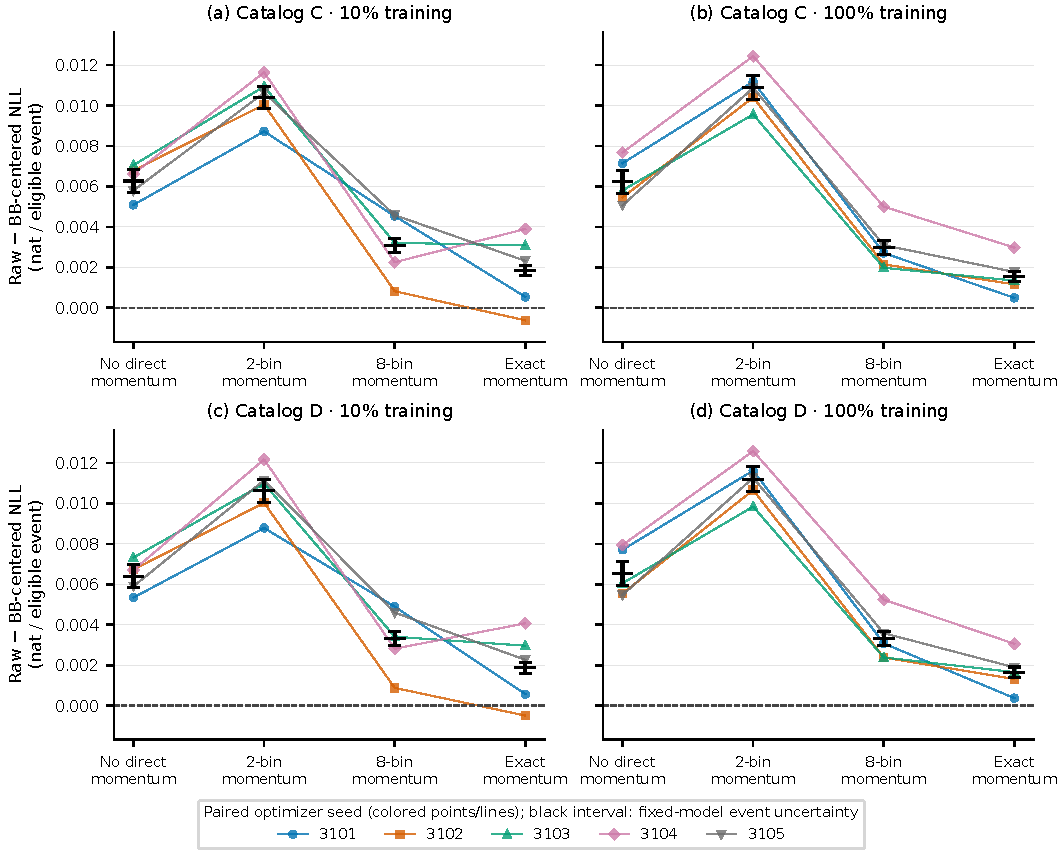
\includegraphics[width=0.92\textwidth]{editorial_figures/information_gain_ladder.pdf}
\caption{Centering gains across four neural information levels. Colored
points retain all five paired optimizer seeds; black intervals are approximate
95\% simultaneous event intervals over 16 contrasts within each catalog.
Lines guide the eye between categorical encodings and do not define an
information-distance scale.}
\label{fig:information_gain}
\end{figure*}

The increase from no direct momentum to two bins is
$0.004127$--$0.004662$ nat/event. It is followed by decreases of
$0.007302$--$0.007908$ from two to eight bins and
$0.001237$--$0.001673$ from eight bins to exact momentum. All simultaneous
intervals exclude zero in these directions. For example, at 100\% training
on C the first difference is $0.004662$ with interval
$[0.004395,0.004929]$, and the next is $-0.007908$ with interval
$[-0.008447,-0.007368]$. The exact-minus-no-direct endpoint is negative,
$-0.004884$ to $-0.004427$. Full tables appear in Supplementary Section S1.

The two-bin peak is stable across all five paired optimizer seeds: each has
the initial rise and the following decline in both catalogs and fractions.
The smaller decrease from eight-bin to exact conditioning occurs in four of
five seeds at 10\% training and all five at 100\%. Leave-one-seed-out means
retain the direction of every reported contrast. At 10\% on C, the final
decline has mean $-0.001237$, seed SD $0.002137$, and omission range
$[-0.001958,-0.000547]$ nat/event. Exact conditioning at 10\% also has
one negative centering-gain seed in each catalog; the other seven settings
favor BB-centered in all five seeds. These seed summaries complement the
conditional event intervals.

\subsection{Exact momentum gives the lowest mean NLL}

For both representations, the five-seed mean absolute NLL decreases in the
order no direct momentum, two bins, eight bins and exact momentum in every
catalog/fraction setting (Fig.~\ref{fig:information_absolute}). BB-centered
without direct momentum remains worse than its exact-momentum counterpart
by $0.019002$--$0.019578$ nat/event. The two-bin condition has the largest
centering gain, yet its absolute NLL is worse than exact conditioning by
$0.005004$--$0.005329$ nat/event. The representation gain and the absolute
mean NLL of the complete predictor therefore select different information levels.

\begin{figure*}[t]
\centering
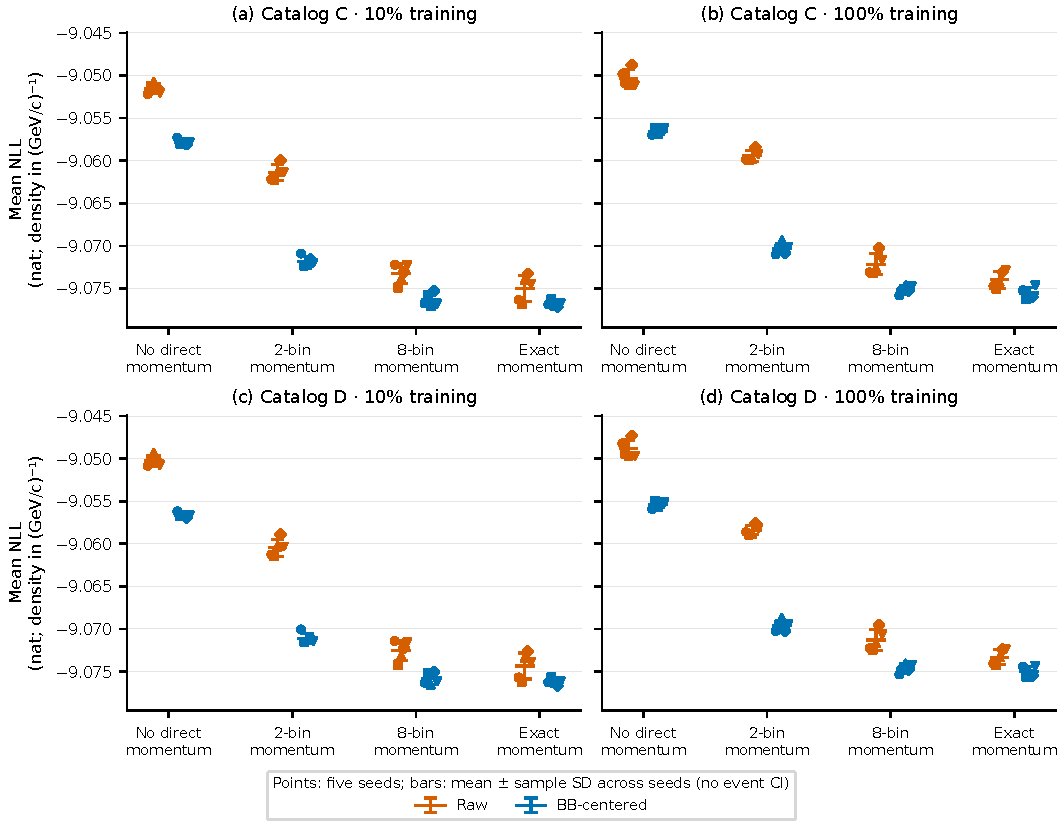
\includegraphics[width=0.92\textwidth]{editorial_figures/information_absolute_nll.pdf}
\caption{Absolute original-unit differential NLL (in GeV/$c$ density units;
more negative values indicate higher likelihood). All five seeds and their
sample SD are shown. These bars describe optimizer variability. Exact momentum
gives the lowest mean NLL for each representation.}
\label{fig:information_absolute}
\end{figure*}

The 10\% models have lower mean NLL than their 100\% counterparts under
the common update budget. This comparison also changes exposure per event;
it describes the specified training procedure rather than an intrinsic
advantage of using fewer data.

Providing two-bin momentum information improves the centered models more
than the raw-target models on average, widening the centering advantage.
Further refinement produces larger mean NLL reductions for the raw-target
models, narrowing that advantage. This relationship holds for the five-seed
means in both catalogs and at both training fractions
(Figs.~\ref{fig:information_gain} and \ref{fig:information_absolute}).

\subsection{Aggregate gains coexist with local losses}
\label{sec:fresh_local}

Positive overall gains conceal negative mean gains within physical groups
(Table~\ref{tab:information_local}). Without direct momentum, 25 and 22 of
42 groups have negative means on C at 10\% and 100\% training, and 27 and
23 on D. Respectively 23, 20, 22 and 20 retain upper bounds below zero after
simultaneous adjustment across all 336 group gains per catalog.
The two-bin condition also has local losses despite its largest overall gain:
13--18 groups have negative means, and nine or ten negative simultaneous bands.
Eight-bin and exact conditioning have fewer negative-mean groups, with most
corresponding intervals including zero.

\begin{table}[t]
\centering
\setlength{\tabcolsep}{2.6pt}
\caption{Counts out of 42 physical groups. ``Mean $<0$'' is descriptive;
``Upper $<0$'' uses the approximate 95\% simultaneous band over all 336 group
gains within that catalog. The C/D coverage families are separate.}
\label{tab:information_local}
\begin{tabular}{llrrrr}
\toprule
 & & \multicolumn{2}{c}{C} & \multicolumn{2}{c}{D} \\
\cmidrule(lr){3-4}\cmidrule(lr){5-6}
Context & Train & Mean$<0$ & Upper$<0$ & Mean$<0$ & Upper$<0$ \\
\midrule
No direct & 10\% & 25 & 23 & 27 & 22 \\
No direct & 100\% & 22 & 20 & 23 & 20 \\
2-bin & 10\% & 18 & 9 & 17 & 9 \\
2-bin & 100\% & 13 & 10 & 14 & 10 \\
8-bin & 10\% & 2 & 0 & 3 & 0 \\
8-bin & 100\% & 6 & 1 & 5 & 1 \\
Exact & 10\% & 3 & 0 & 1 & 0 \\
Exact & 100\% & 9 & 0 & 9 & 1 \\
\bottomrule
\end{tabular}
\end{table}

Figure~\ref{fig:information_local} shows all groups for C without direct
momentum at 100\% training. The complete set of 16 group displays and
their numerical summaries accompanies the companion repository. Groups with
negative means contain about 52--64\% of eligible events in the no-direct
condition. This measures the event share of those groups, not how many
individual events have worse scores.

\begin{figure*}[t]
\centering
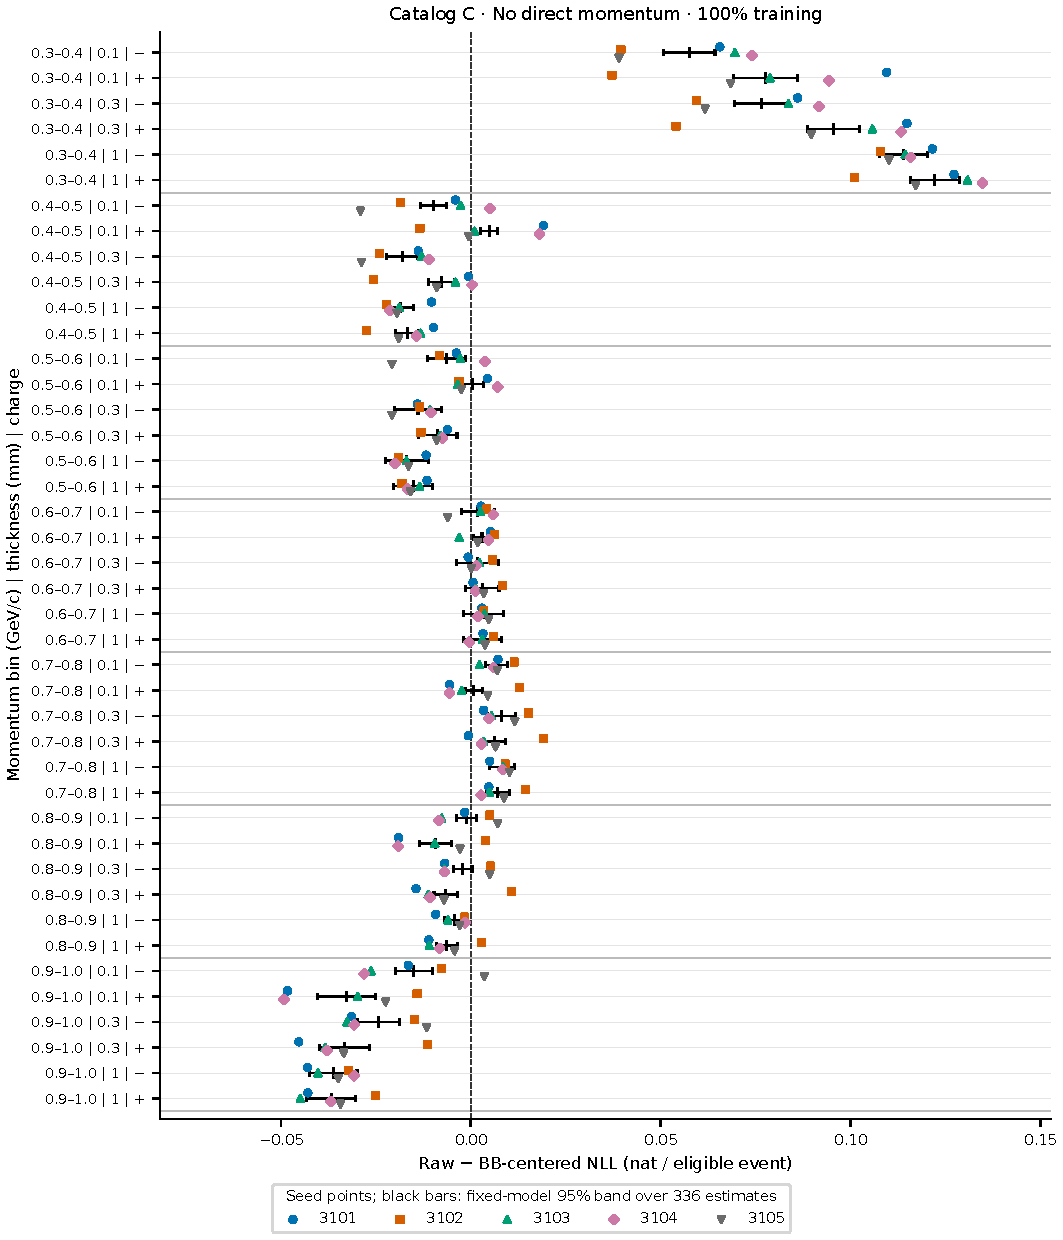
\includegraphics[width=0.84\textwidth]{editorial_figures/information_local_C_Hidden5_f100.pdf}
\caption{All 42 physical-group gains for No direct momentum at 100\% training on fresh C.
Colored symbols show five paired optimizer seeds; black ticks show their mean
and black bars give simultaneous intervals over the $8\times42=336$
context/fraction-by-group estimates within C. The overall gain is positive although
20 group intervals lie below zero. No local-sign filter is applied.}
\label{fig:information_local}
\end{figure*}

\subsection{Secondary fitted-center comparisons}
Under exact conditioning, BB-centered improves mean NLL over Raw at both
capacities and all three fractions on each fresh catalog. Linear centering
also improves all six means per catalog. The six polynomial-ridge-minus-BB
NLL contrasts favor BB-centered. Individual seed exceptions remain in the
complete C/D summaries (Supplementary Section S3). Improvement over Raw is
therefore also attainable with a training-fitted center.

\section{Residual-location and conditional-calibration diagnostics}
\label{sec:diagnostics_main}

The source diagnostic finds lower remaining momentum-\allowbreak location variation
after BB centering at each incomplete-\allowbreak information level. In units of
$10^{-10}\,(\mathrm{GeV}/c)^2$, Raw and BB-centered burdens are respectively
$1.577$ and $1.222$ without direct momentum, $1.543$ and $1.176$ with two
bins, and $0.931$ and $0.906$ with eight bins. The reduction is slightly
largest at two bins and much smaller at eight bins, consistent with the broad
gain pattern. Figure~\ref{fig:location} plots their square roots; the common
original-unit statistic is shown once.

\begin{figure*}[t]
\centering
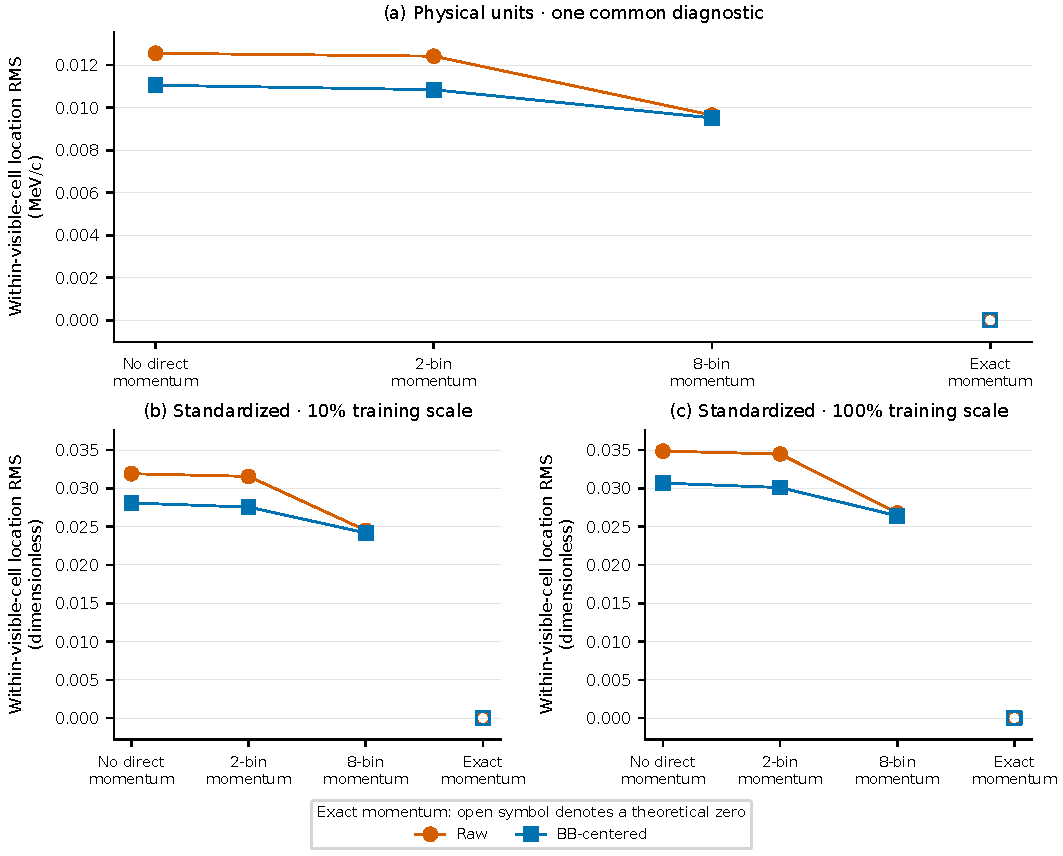
\includegraphics[width=0.88\textwidth]{editorial_figures/information_source_location.pdf}
\caption{Source residual-location burden from the 56-bin common refinement.
The square root of the event-weighted within-cell residual-mean variance is
shown once in MeV/$c$ using the saved 100\% preprocessing record, and
separately in each fraction's standardized units.
Exact momentum is the theoretical zero endpoint for unobserved-momentum
burden.}
\label{fig:location}
\end{figure*}

At 100\% training without direct momentum input, the mean gain on catalog C
is positive in the lowest momentum interval ($0.3$--$0.4$ GeV/$c$;
$+0.0905$ nat/event) but negative in the highest interval
($0.9$--$1.0$ GeV/$c$; $-0.0297$ nat/event), with the same signs on D.
Saved original-unit residual medians are consistent with this regional sign
flip, although the present frozen comparisons do not quantify what share of the
two-bin peak arises from location drift alone. Across C/D and both charges over
$0.6$--$1.0$ GeV/$c$, the Raw residual median $Y-\mu$ plateaus at $t=1.0$ mm
($+124.9$ to $+130.8$ keV/$c$, varying by $\leq4.3$ keV/$c$ within each
catalog--charge series), whereas $c_{\mathrm{BB}}$ rises from its $0.555$
GeV/$c$ minimum ($410.0$ keV/$c$) to $426.3$ keV/$c$ at $1.00$ GeV/$c$ as
$T_{\max}$ grows from $15.7$ to $49.8$ MeV ($4.6$ to $49.8$ MeV over
$0.30$--$1.00$ GeV/$c$) and $-\delta(\beta\gamma)/2$ is omitted. Subtracting
$c_{\mathrm{BB}}$ therefore imparts a monotonic downward drift to the bulk
residual median across $0.6$--$1.0$ GeV/$c$ ($-85.9$ to $-104.3$ keV/$c$ at
$t=1.0$ mm, and $-67.2$ to $-104.3$ keV/$c$ over $0.3$--$1.0$ GeV/$c$); the
$0.1$ and $0.3$ mm slabs show the same thickness-scaled pattern. Detailed
density-term accounting is given in Supplementary Section S2.2.

Predictive quantile diagnostics reveal corresponding regional trade-offs. Without
direct momentum at 100\% training, the fraction below the predicted median
in the lowest momentum interval moves from $0.317$--$0.319$ for Raw to
$0.398$--$0.399$ for BB-centered across C/D, closer to the nominal $0.5$.
In the highest interval it moves from $0.553$--$0.559$ to
$0.582$--$0.587$, farther from $0.5$, while predictive interquartile
coverage falls from $0.478$--$0.479$ to about $0.435$. These descriptive
five-seed means show that aggregate likelihood improvement can accompany
worse regional location and spread calibration.

\section{Discussion}
\label{sec:discussion}

The central finding is a two-bin peak in relative centering benefit that
persists across all five paired seeds in the tested design. Exact momentum
gives the lowest mean NLL, while improvements averaged over the catalog
coexist with local losses. Relative centering benefit, absolute prediction
quality and the distribution of gains across physical conditions therefore
describe complementary aspects of this measured interaction. A prescribed representation does not simply compensate
for missing neural inputs. Its value depends on how its encoded information
interacts with the information and flexibility remaining in the conditional
density estimator. The controlled information ladder exposes this interaction
without requiring a new centering method.

The model-family analysis explains why complete-condition invertibility is
compatible with different finite-model performance. A physical translation
prescribes part of the momentum dependence, leaving the flow to model the
residual structure. Each representation's remaining location burden decreases
under information refinement, while the difference between burdens can vary
non-monotonically. The source diagnostic provides a concrete example of this
distinction. Interventions on the center or residual family would help
separate location effects from residual scale, shape and optimization effects.

\paragraph{Physical reference and fitted centering.}
Bethe--Bloch describes mean electronic energy-loss rate, whereas our target
is an individual event's momentum loss conditional on an eligible
exit~\cite{Bichsel1988,PDG2025}. Momentum loss, local energy deposition and
detector ionization signal are related but distinct
observables~\cite{Bichsel2006}. In thin silicon, rare high-transfer $\delta$
electrons drive the relativistic rise of $S_{\mathrm{BB}}$ while the
Landau--Vavilov--Bichsel bulk remains nearly flat above minimum ionization,
compounded by the omitted silicon density effect. The observed regional
likelihood and calibration patterns are consistent with this mismatch: under
no-direct conditioning, a single residual distribution per $(t,q)$ must
accommodate both steep $1/\beta^2$ behavior below $0.55$ GeV/$c$ and the
downward high-momentum residual drift above $0.6$ GeV/$c$, whereas the two-bin
split at $0.65$ GeV/$c$ separates these regimes with one bit of momentum
information while preserving continuous $1/\beta^2$ centering within
$[0.3,0.65)$. At eight-bin and exact conditioning, Raw can resolve the
low-momentum curve directly without incurring high-momentum over-subtraction.
While the present frozen comparisons cannot isolate how much of the two-bin
peak comes from this location drift relative to residual scale, shape or
optimization dynamics, they show that physical knowledge reshapes the residual
learning problem in a regime-dependent manner.

The linear center's improvement under exact conditioning also establishes
the relevance of general target centering. Its coefficients and those of the
polynomial-ridge center use source-training data; BB centering instead uses
physical constants and a fixed stopping-power expression. Their construction
costs differ even when flow capacity is matched. These fitted centers were
not evaluated across the four-level ladder. The observed non-monotonicity
belongs to this physical center in this design; it has not been shown to be
unique to Bethe--Bloch information or common to all reasonable centers.

\paragraph{Practical significance.}
For paired event densities,
$\Delta=N^{-1}\sum_i\log[p_{\rm BB}(y_i\mid x_i)/p_{\raw}(y_i\mid x_i)]$
implies a geometric-mean density ratio $\exp(\Delta)$. With seed averaging,
the mean also runs over event--seed pairs. The exact-momentum gains correspond
to about $0.16$--$0.19\%$ higher geometric-mean assigned density, compared
with $1.05$--$1.13\%$ for two bins. These small per-event effects should be
considered alongside absolute scores and regional calibration. Downstream
reconstruction, simulation error, speed and the cost of maintaining the
center were not evaluated.

\paragraph{Scope and limitations.}
The conclusions concern one pion--silicon transport setup, one principal
Small flow architecture (width 32 across the four-level ladder, with width 128
tested only under exact conditioning), one pooled target scale and two training
fractions under a fixed 20,000-update budget (about 171 epochs at 10\% versus
17.1 epochs at 100\%, characterizing finite-budget approximation rather than
asymptotic convergence). Deploying such flows as multi-layer generative track
simulators would additionally require enforcing $Y\geq0$ (avoiding the
$0.035\%$--$0.114\%$ untruncated $Y<0$ tail mass), thickness-aware scaling, and
non-identity heavy-tail parameterizations beyond $|z|>8$ (where the frozen RQS
reverts to a fixed-scale logistic tail; across the primary models, observed
maxima reach $z_{\max}=104.60$--$114.70$ on C and $87.09$--$95.78$ on D, with
$0.15\%$--$0.19\%$ of eligible events lying at $z>8$ and none below $-8$,
Supplementary Section S4.2).
Fresh C/D measure new event sampling within this setup; they do not test
another material, physics list or out-of-range distribution. Event intervals
condition on selected models, and the five optimizer seeds share one source
catalog, leaving training-data uncertainty unmeasured. Location and quantile
diagnostics are descriptive; the coordinate-dependent likelihood accounting
does not identify a unique causal decomposition into location, scale and
shape. Group summaries can also conceal finer conditional errors. These
limits define the domain in which the observed interaction can be assessed.

\section{Conclusion}
\label{sec:conclusion}

For the tested pion momentum-loss models, physical target centering improves
mean NLL at all four neural information levels, with its largest relative
gain at two-bin momentum. Exact momentum nevertheless gives the lowest mean NLL, and aggregate gains do not ensure improvement throughout the
physical domain. The central two-bin peak persists across all five paired
seeds, whereas the smaller final decline is less stable at 10\% training.
Evaluating a prescribed representation therefore requires distinguishing its
relative gain from the absolute performance and conditional behavior of the
complete predictor.

% Optional acknowledgements block may be uncommented by the authors if applicable:
% \begin{acknowledgements}
% \end{acknowledgements}

\section*{Data Availability Statement}
All aggregate seed and physical-group summaries, saved 2000-draw paired
bootstrap resamples, predictive and residual diagnostic summaries, frozen
protocol manifests, run manifests and cryptographic SHA-256 checkpoint digests
supporting the tables, figures and intervals in this article and the Electronic
Supplementary Material are openly archived in the companion GitHub repository at
\url{https://github.com/xschang1002/EPJC} (release tag \texttt{v1.0.0-epjc}).
The uncompressed raw Geant4 event ledgers, binary PyTorch checkpoints and
per-event score arrays ($\simeq 62$~GiB), verified against the cryptographic
SHA-256 manifests published in the repository, are archived locally and are
available from the corresponding author upon reasonable request.

\section*{Code Availability Statement}
The spline-flow training, Geant4 simulation interface, frozen catalog scoring,
statistical analysis, unit-test suite and isolated aggregate-reproduction
scripts are openly archived in the companion GitHub repository at
\url{https://github.com/xschang1002/EPJC} (release tag \texttt{v1.0.0-epjc}),
together with cross-platform and pinned environment dependency specifications
(see Supplementary Section S4).

\section*{Declarations}
\paragraph{Funding.}
The authors declare that no funds, grants, or other support were received during
the preparation of this manuscript.

\paragraph{Competing interests.}
The authors have no relevant financial or non-financial interests to disclose.

\paragraph{Author contributions.}
X.~Chang: Conceptualization, Methodology, Software, Formal analysis, Validation,
Writing -- original draft. Y.~Xiao and C.~Song: Methodology, Validation,
Writing -- review \& editing. All authors read and approved the final
manuscript.

\paragraph{Use of AI-assisted tools.}
AI-assisted coding and scientific-writing tools were used during verification
scripting, structural editing and template preparation. The authors reviewed
and verified all source code, numerical results, citations and scientific
statements, and take full responsibility for the content of this publication.

\begingroup
\raggedright
\bibliographystyle{spphys}
\bibliography{references}
\endgroup

\end{document}
